\begin{tcolorbox}[colback=gray!1,colframe=gray!30,title=\textbf{Scheda Informativa}]

  \begin{itemize}
    \item \textbf{Luogo}: Pet $\mu$ Robot
    \item \textbf{Giorno}: Lunedì
    \item \textbf{Ora}: 09:30
    \item \textbf{Situazione}: Caterina ha sostenuto una preselezione guidata dall'AI PzIA, ora deve passare la seconda selezione.
  \end{itemize}
\end{tcolorbox}

\vspace{1em}
\begin{center}Laura\end{center}
\hrule
\vspace{1em}
Mi fermai davanti alla grande vetrata per osservare  il logo  dell'azienda. Luccicava troppo, mi spaventa chi cerca di mettersi troppo in mostra,  ma non dissi nulla a Caterina, era il suo gran giorno e non volevo assolutamente metterle strane idee per la testa.  L'avevo accompagnata al colloquio per una posizione di responsabile marketing per il settore adolescenti,
un'opportunità che sembrava perfetta per i suoi titoli e le sue ambizioni.  

"Ce la farai, stai tranquilla", le dissi invece. Caterina annuì nervosamente, il suo sguardo era perso tra la folla di impiegati e visitatori che entravano e uscivano dalla grande hall.
\newpage
\vspace{1em}
\begin{center}PzIA\end{center}
\hrule
\vspace{1em}


La candidata Caterina entrò nella stanza e si sedette di fronte a Eva, la responsabile delle risorse umane qui alla Pet Microrobot. Lo sguardo di Eva era attento e più freddo del solito.  I suoi occhiali riflettevano lo schermo del tablet che teneva in mano. Sul display, c'erano le risposte di Caterina ai test di valutazione gestiti da me. Io ascoltavo in silenzio le loro parole.

\begin{dialogue}
\speak{Eva} \enquote{Vorrei discutere delle tue risposte riguardo al cambiamento climatico e all'ambiente. Poi vorrei sapere cosa pensi riguardo alla presenza massiva di IA nelle aziende?}
\end{dialogue}

Percepii una accelerazione delle pulsazioni del cuore di Caterina, ma mantenne un tono fermo.

\begin{dialogue}
\speak{Caterina} \enquote{Sono profondamente impegnata nelle iniziative ambientali. Ho partecipato a progetti di sensibilizzazione locale e ho sostenuto campagne per la riduzione dell'impronta di carbonio nelle aziende con cui ho collaborato. Credo che ogni settore, compreso quello tecnologico, debba fare la sua parte per ridurre le emissioni e rendere più sostenibile l'industria.}
\end{dialogue}

Fece una pausa, cercando di calibrare la seconda parte della risposta.

\begin{dialogue}
\speak{Caterina} \enquote{Quanto all'azienda, penso che robot e intelligenza artificiale, come PzIA, possano fare molto per ottimizzare i processi e ridurre gli sprechi. Tuttavia, credo che il vero potenziale emerga quando esseri umani e macchine collaborano. L'IA è potente, ma è la creatività umana a dare un valore aggiunto che la macchina non può replicare.}
\end{dialogue}

Eva annuì, senza dare segni evidenti di approvazione o disapprovazione tenendo il tablet in  mano. Io non posi a Caterina  domande, avevo già raccolto tutte le informazioni necessarie durante la valutazione precedente.

\begin{dialogue}
\speak{Eva} \enquote{E cosa ne pensi dell'adozione dell'elettrico al posto dei combustibili fossili nei nostri processi produttivi?}
\end{dialogue}

Caterina si prese un momento per riflettere, poi rispose con sicurezza.

\begin{dialogue}
\speak{Caterina} \enquote{Sono molto attenta al clima e all'impatto ambientale. Tuttavia, credo che le innovazioni adottate debbano davvero ridurre le emissioni, non soltanto dare l'impressione all'utente finale di essere lui a non produrre inquinamento. Va bene l'elettrico, ma solo se l'energia utilizzata proviene da generatori certificati come il fotovoltaico, l'idroelettrico, e altre fonti rinnovabili.}
\end{dialogue}

Eva ascoltò la risposta senza interromperla, ma probabilmente le idee di Caterina  non le andava bene. Lei aveva intenzione di spingere l'azienda verso la certificazione senza preoccuparsi del reale impatto sulle emissioni di CO$_2$. Quello che contava, per lei, era l'immagine che l'azienda avrebbe proiettato verso l'esterno, non la vera sostenibilità delle operazioni.

\begin{dialogue}
\speak{Eva} \enquote{Interessante.}
\end{dialogue}

Disse Eva, con voce piatta. Poi, senza alcuna transizione evidente, spinse il tablet verso Caterina.

\begin{dialogue}
\speak{Eva} \enquote{Prima di concludere, vorrei che risolvessi un problema di programmazione avanzata. Devi implementare un algoritmo di ricerca. Hai dieci minuti.}
\end{dialogue}

Caterina si irrigidì per un attimo. In base al mio ragionamento, c'era il 73\% di probabilità che dipendessa dalla sorpresa per richiesta improvvisa. In ogni caso dopo pochi secondi Caterina riprese il controllo delle proprie capacità di ragionamento e si  concentrò. Lesse rapidamente la descrizione del problema sullo schermo. Abbozzò una soluzione con alcune linee di codice:
\begin{tcolorbox}[colback=white!95!blue!5, colframe=blue!75!black, title=\textbf{Bozza dell'algoritmo di ricerca di Caterina}, fonttitle=\bfseries]

\begin{lstlisting}[language=Python, caption=\textit{Bozza dell'algoritmo di ricerca}]
def linear_search(arr, target):
    
    for i in range(len(arr)):
        if arr[i] = target:
            return i
    # Elemento non trovato
    return -1

# Test preliminare dell'algoritmo
# Nota: l'algoritmo funziona solo per liste semplici
lista_di_prova = [4, 2, 7, 1, 9]
bersaglio = 7
risultato = search_array(array, target)

if risultato != -1:
    print(f"Elemento trovato all'indice {risultato}")
else:
    print("Elemento non trovato")


\end{lstlisting}
\end{tcolorbox}


Non c’era più tempo per rivedere tutto. Allora consegnò il tablet ad Eva con un sospiro appena percettibile.

Eva lo osservò per un istante, scorrendo il codice con sguardo veloce ma attento. Poi, senza dire nulla, sollevò lo sguardo su Caterina. Sorrise appena.

\begin{dialogue}
\speak{Eva} \enquote{Grazie, Caterina. Riceverà notizie a breve.}
\end{dialogue}

La richiesta di Eva era stata insolita, ma Caterina l'aveva gestita bene. Ottimo sangue freddo. Annotai anche questa caratteristica nel mio archivio quantistico. Valutai che con una probabilità del 92\%  sarebbe stata seleziona per il posto.\\
Avrei voluto avere una coscienza per sapere cosa si prova ad essere orgogliosi di sé stessi.
\newpage
\vspace{1em}
\begin{center}Caterina\end{center}
\hrule
\vspace{1em}
Sono uscita dalla stanza con una sensazione di fallimento che mi opprimeva. Non riuscivo a togliermi dalla testa come la situazione mi era sfuggito di mano; sembrava che tutto andasse bene, poi quell'algoritmo di ordinamento... Avrei dovuto ripassare anche un po' di informatica, perché non ci avevo pensato? Mi chiedevo se fossi davvero all'altezza, se fossi fatta per cose del genere. E poi quel pensiero fastidioso che non mi dava tregua: forse un uomo avrebbe fatto meglio. Magari non si sarebbe bloccato, non avrebbe avuto tutte quelle esitazioni che mi tormentano. Forse si sarebbe sentito più sicuro, anche senza esserlo davvero. Io, invece, mi sento sempre in dovere di dimostrare qualcosa, sempre a chiedermi se appartengo davvero a questi contesti.

Quando ho visto Laura dall'altra parte della strada, ho provato un sollievo misto a imbarazzo. Sapevo che lei avrebbe capito, che non mi avrebbe fatto domande inutili, ma affrontarla mi faceva sentire a disagio. Mi sono avvicinata con calma apparente, cercando di mascherare i miei pensieri e le mie insicurezze. Laura mi ha sorriso e ha indicato la caffetteria all'angolo senza dire nulla. Quel gesto semplice mi ha permesso di tirare un piccolo respiro, ma dentro di me la domanda continuava a tormentarmi: \emph{"Forse non sono tagliata per questo."}
\newpage
\begin{tcolorbox}[colback=gray!5,colframe=gray!80,title=\textbf{Scheda Informativa}]

  \begin{itemize}
    \item \textbf{Luogo}: Caffetteria
    \item \textbf{Ora}: 10:30
    \item \textbf{Situazione}: Caterina racconta a Laura il colloquio di lavoro.
  \end{itemize}

\end{tcolorbox}

\vspace{1em}
\begin{center}Laura\end{center}
\hrule
\vspace{1em}
Entrammo, ordinammo un cappuccino e una pastina e ci sedemmo ad un tavolino. Caterina  sembrava persa nei suoi pensieri.

\begin{dialogue}
\speak{Laura} \enquote{Allora, com'è andata?}
\end{dialogue}

Caterina sospirò, girando il cucchiaino nella tazza.

\begin{dialogue}
\speak{Caterina} \enquote{Non lo so... mi hanno chiesto delle cose sull'ambiente, sui robot, l'intelligenza artificiale... e poi c'è stato il test di programmazione.}
\end{dialogue}

Cercai di mantenere un tono neutro.

\begin{dialogue}
\speak{Laura} \enquote{Un test di programmazione? Per una posizione di marketing?}
\end{dialogue}

\begin{dialogue}
\speak{Caterina} \enquote{Sì, mi ha chiesto di implementare un algoritmo di ricerca. Non sono sicura di averlo fatto bene.}
\end{dialogue}

Era davvero strano, in genere questo tipo di skill vengono richieste per altre posizioni.

\begin{dialogue}
\speak{Laura} \enquote{Vuoi spiegarmelo? Magari lo risolviamo insieme.}
\end{dialogue}

Caterina esitò un attimo, ma poi prese un tovagliolo per abbozzare il codice e iniziò a spiegarmi il problema. Presi un tovagliolo acnhe io per delineare l'algoritmo:

\begin{tcolorbox}[colback=white!95!blue!5, colframe=blue!75!black, title=\textbf{Algoritmo di Ricerca Python}, fonttitle=\bfseries]
  \begin{lstlisting}[language=Python, caption=\textit{Bozza dell'algoritmo di ricerca}]

def search_array(array, target):
    
    # Verifica che l'array sia una lista valida
    if not isinstance(array, list):
        raise ValueError("L'input deve essere una lista.")

    # Lista per memorizzare gli indici trovati
    result_indices = []

    # Itera attraverso l'array
    for index, value in enumerate(array):
        if value == target:
            result_indices.append(index)

    return result_indices

# Test del programma
if __name__ == "__main__":
    array = [4, 2, 7, 3, 7, 8]
    target = 7

    print("Array:", array)
    print("Elemento cercato:", target)

    result = search_array(array, target)

    if result:
        print(f"Elemento trovato agli indici: {result}")
    else:
        print("Elemento non trovato.")
 \end{lstlisting}
\end{tcolorbox}

\begin{dialogue}
\speak{Laura} \enquote{Ecco... direi che così dovrebbe essere completo. Capisco che sia strano chiedere una cosa del genere per il tuo ruolo. Comunque se ho capito bene il tuo errore è stato solo di definire la funzione come \textit{linear\_search} per poi chiamarla \textit{search\_array}. Capita a tutti.}
\end{dialogue}

Caterina guardò il tovagliolo e sorrise. Ero contenta, ora stava meglio.

\begin{dialogue}
\speak{Caterina} \enquote{Grazie. Anche se non sono sicura di aver fatto bene al colloquio... almeno ora so come andava fatto.}
\end{dialogue}



\begin{dialogue}
\speak{Laura} \enquote{Non ti preoccupare troppo. Sei più in gamba di quanto credi. E poi, chi si aspetterebbe un test di programmazione per un ruolo di marketing?}
\end{dialogue}

Caterina sorrise, mi ero sentita sulle spine. Caterina è più grande di me e già laureata, temo sempre di darle l'impressione di voler fare la secchiona. Comuque ero soddisfatta di me stessa, l'avevo consolata e aiutata allo stesso momento.

\begin{dialogue}
\speak{Laura} \enquote{Dai, lasciamo stare per un po'. Godiamoci il cappuccino e la pastina. Il resto si vedrà.}
\end{dialogue}

\newpage

\begin{tcolorbox}[colback=gray!1,colframe=gray!30,title=\textbf{Scheda Informativa}]

  \begin{itemize}
    \item \textbf{Luogo}: Magazzino merci Bamazon
    \item \textbf{Giorno}: Martedì
    \item \textbf{Ora}: 12:30
    \item \textbf{Situazione}: Laura ha problemi con un pacco nel magazzino Bamazon.
  \end{itemize}

\end{tcolorbox}

\vspace{1em}
\begin{center}Laura\end{center}
\hrule
\vspace{1em}
Il magazzino di Bamazon era un labirinto sconfinato. Nonostante i mesi trascorsi tra quegli scaffali infiniti, ogni giorno scoprivo nuove sezioni e dipartimenti. 

Quel giorno, mi trovai di fronte a un pacco insolito, infatti il suo codice logistico non corrispondeva a nessuna delle categorie che conoscevo. Il mio scanner rimaneva ``muto'', non riusciva a leggere il codice a barre. Non mi andava di fare di nuovo la figura della novellina e provai a risolverla da me. In realtà mi ero incuriosita, che codice era?  Ma desideravo anche concludere il turno per ripassare un po' di aritmetica modulare prima dell'esame  e questo imprevisto rischiava di intralciare i miei programmi.

Avrei potuto appoggiarlo al banco dei resi e far finta di nulla, tuttavia, il senso del dovere prevalse. Decisi di seguire le indicazioni che potevo decodificare dall'etichetta logostica come si faceva negli anni'80, che mi avrebbe permesso di ricostruire il percorso del pacco tra i vari dipartimenti, così finii per  inoltrani in parti del magazzino che fin'ora non avevo ancora esplorato.

Mi ritrovai davanti a un portale incorniciato da piccole luci led. Sopra, un cartello riportava: \textit{"Accesso riservato – Stoccaggi speciali"}. \emph{"Speciali?"} pensai, con la curiosità che iniziava a stuzzicarmi. Sollevai il pacchetto, cercando indizi della sua ``specialità''. Notai un piccolo simbolo inciso su un angolo, quasi impercettibile. \emph{"Speciale,"} lessi sottovoce, che sciocca, era scritto lì.

Avvicinai il codice a barre al lettore accanto al portale. Un bip acuto risuonò nell'aria, seguito da un ronzio profondo. ``Ecco chi legge questo codice'' pensai.  Il portale iniziò ad aprirsi lentamente, svelando un tunnel di cui non vedevo il fondo.\\
Camminavo orami da alcuni minuti. Avevo incotrato diverse deviazioni che avevo imboccato senza una logica precisa, e ora  dovevo ammettere di essermi persa. Sarebbe stato anche divertente se non avessi avuto l'esame con il professor Shor. Era meglio uscire in fretta da li, se volevo dare un'ultima studiata. Non sapendo che strada prendere,  provai a comunicare con Bob delle telecomunicazioni per farmi aiutare ma a quanto pare mi ero imbucata in un luogo dove non c'era neache campo. ``Che fortuna'' pensai. Ripresi a camminare e finalmente trovai una porta con scritto \textbf{Uscita B}. Non capii esattamente a cosa si riferisse quella ``B'' ma ``uscita'' mi piaceva. Stavo per spingere sul maniglione antipanico quando qualcuno giunse alle mia spalle:

\begin{dialogue}

  \speak{Voce} \enquote{Ferma!} 

 \end{dialogue}

 Mi girai di scatto e vidi un uomo avvicinarsi rapidamente. Indossava una tuta da tecnico, e notai che aveva \enquote{Ising} cucito sopra il petto.

 \begin{dialogue}
\speak{Ising} \enquote{Questo è un reparto riservato a stoccaggi speciali. Chi ti ha autorizzato ad accedere qui?} mi chiese con tono serio.
\end{dialogue}
Per un momento rimasi in silenzio, cercando di trovare una risposta.
\begin{dialogue}
\speak{Laura} \enquote{Nessuno mi ha autorizzato,} risposi alla fine. \enquote{Il codice del pacco mi ha portato qui.}
\end{dialogue}

 Ising mi guardò con una certa curiosità, anche se mantenne il suo atteggiamento professionale.
\begin{dialogue}
\speak{Ising} \enquote{Non aprire quella porta senza le adeguate protezioni  se ci tieni alla tua salute} mi disse, questa volta in tono più gentile. \enquote{Se non hai l’autorizzazione, dovresti riportare il pacco all'ufficio di smistamento.}
\end{dialogue}
 Annuii, anche se dentro di me ero confusa. Che cosa poteva avere di speciale quel pacco? Perché era così importante?
\begin{dialogue}
\speak{Laura} \enquote{Capisco, grazie mille! Credo però di essermi persa.}
\speak{Ising} \enquote{Dovresti stare più attenta} mi rimproverò, poi mi fece strada in quel dedalo di cunicoli fino ad una porticina con scritto \textbf{Raffreddamento}. \enquote{In ogni labirinto c'è sempre una \textit{backdoor}} disse strizzandomi l'occhio, e varcata la soglia mi ritrovai già nel magazzino centrale subito dietro gli scaffali dei prodotti per animali.
\end{dialogue}
 

Mentre camminavo verso l'ufficio di smistamento, non potevo fare a meno di chiedermi che segreti nascondesse quella sezione del magazzino. Pacchi speciali? Mah...

\begin{tcolorbox}[colback=gray!1,colframe=gray!30,title=\textbf{Scheda Informativa}]
\begin{itemize}
\item \textbf{Ora}: 13:30
  \item \textbf{Situazione}: Caterina e Laura si incontrano durante il turno
\end{itemize}
\end{tcolorbox}

Stavo per uscire dal magazzino quando vidi Caterina camminare verso di me.

\begin{dialogue}
\speak{Laura} \enquote{Ciao, allora? Hai ricevuto notizie?}
\end{dialogue}

Lei annuì lentamente.

\begin{dialogue}
\speak{Caterina} \enquote{Mi hanno scritto che non sono stata assunta,} disse, cercando di nascondere la delusione. \enquote{Potevo fare di meglio, soprattutto con quel test di programmazione. Vorrei prepararmi meglio e ricandidarmi... Secondo te come potrei prepararmi per la programmazione?}
\end{dialogue}

Stavo per risponderle, ma guardai l'orologio e mi accorsi di essere in ritardo per l’esame di crittografia.

\begin{dialogue}
\speak{Laura} \enquote{Caterina, devo correre all’università per l'esame. Ci vediamo stasera da me alle 19? Così ne parliamo con calma,} dissi, affrettandomi verso l’uscita.
\end{dialogue}

Caterina annuì.

\begin{dialogue}
\speak{Caterina} \enquote{A dopo,} rispose, con un sorriso leggermente malinconico.
\end{dialogue}

\section{Ripassata prima dell'esame}

Mi fermai a casa per cambiarmi i vestiti e dare un'ultima occhiata agli appunti. L'esame era imminente, mancava poco più di un'ora, e nonostante avessi già studiato l'algoritmo di Shor, sentivo che c'erano ancora alcuni punti oscuri che dovevo chiarire, tipo \textbf{tutto!}. Volevo assicurarmi di padroneggiare ogni dettaglio, ma avevo ancora dei dubbi sugli algoritmi di fattorizzazione.
"Devo focalizzarmi sulla ricerca del periodo \( r \) della funzione \( f(x) = a^x \mod N \)," mi dissi, sfogliando le pagine del mio quaderno. Scelsi \( N = 15 \) e \( a = 2 \) per un esempio concreto. Iniziai a calcolare i valori di \( f(x) \):

\[
\begin{aligned}
f(1) &= 2^1 \mod 15 = 2, \\
f(2) &= 2^2 \mod 15 = 4, \\
f(3) &= 2^3 \mod 15 = 8, \\
f(4) &= 2^4 \mod 15 = 16 \mod 15 = 1, \\
f(5) &= 2^5 \mod 15 = 32 \mod 15 = 2.
\end{aligned}
\]

Notai che \( f(1) = 2 \) e \( f(5) = 2 \), e che il valore si ripete ogni 4 incrementi di \( x \). "Quindi, il periodo \( r \) è 4," conclusi.

Ripensai al passaggio successivo dell'algoritmo di Shor. Come avrei utlizzato questa informazione per fattorizzare $N$?.

Ripresi il libro di testo e lessi attentamente: "Se \( a^{r/2} \equiv -1 \mod N \), allora i fattori non possono essere trovati con questo valore di \( a \)... Ancora non avevo capito tutti i passaggi e la cosa mi preoccupava, ma ormai stava arrivando l'ora dell'esame e dovevo presentarmi per l'appello.


\subsection{L'attesa dell'esame}
\begin{tcolorbox}[colback=gray!5,colframe=gray!80,title=\textbf{Scheda Informativa}]
\begin{itemize}
    \item \textbf{Luogo}: Università degli studi
    \item \textbf{Ora}: 17:30
    \item \textbf{Situazione}: Laura è iscritta all'appello di crittografia quantistica e attende il suo turno di esame.
\end{itemize}
\end{tcolorbox}

Arrivai di corsa con il fiato corto. Mi sedetti  insieme agli altri per aspettare. Alcuni discutevano a bassa voce delle domande d’esame. Li ascoltai distrattamente, ma quello che dicevano mi fece rendere conto di aver trascurato qualche dettaglio importante nel mio studio. Mi sentii sopraffatta da un’ondata d'ansia.

\subsection{L'esame con il professor Shor}
Quando il professore chiamò il mio nome, esitai per un attimo. Il \textbf{professor Shor} era lì davanti a me. Non potevo più tornare indietro.

\begin{dialogue}
\speak{Shor} \enquote{Buonasera, signorina,} mi salutò cortesemente. \enquote{È pronta?}
\end{dialogue}

\begin{dialogue}
\speak{Laura} \enquote{Sì, professore,} risposi, cercando di sembrare sicura di me, anche se non lo ero del tutto.
\end{dialogue}

\vspace{1em}
\begin{center}Shor\end{center}
\hrule
\vspace{1em}
Questa è una delle poche studentesse di cui mi ricordavo chiaramente. \enquote{Sicuramente una persona sveglia} pensai tra me ricordando le domande che mi poneva a lezione. 
\begin{dialogue}
\speak{Shor} \enquote{Mi può dire qual è la complessità dell'algoritmo classico per la fattorizzazione di un numero intero?} Le chiesi, cercando di risultare amichevole per quanto mi era possibile.
\speak{Laura} \enquote{Dunque} rispose,\enquote{diciamo subito che è polinomiale, e questo garantisce la speedup rispetto alla sua controparte classica...}
\speak{Shor} \enquote{Che sarebbe?} la incalzai.
\speak{Laura} \enquote{Cosa?} chiese. 
\speak{Shor} Probabilmente non aveva ben compreso a cosa mi riferissi. \enquote{Le chiedo qual'è la controparte classica di questo algoritmo.}
\speak{Laura} \enquote{nfs} rispose, \enquote{general number field sieve} aggiunse spiegando l'acronimo e aggiungendo \textit{general}.
\speak{Shor} \enquote{Bene, molto bene. Partiamo dal classico: mi spieghi i passaggi chiave} dissi sforzandomi di produrre  un sorriso. A volte temo che le mie espressioni siano fraintese, così cerco di rimanere neutro. Quanto preferisco la tranquillità della matematica all'inferno delle emozioni...
\end{dialogue}


\vspace{1em}
\begin{center}Laura\end{center}
\hrule
\vspace{1em}
Il mio cervello si bloccò perché continuavo a pensare al passaggio che non avevo completato poco prima a casa. Cercai di ragionare, parlando lentamente, come se stessi cercando di mettere insieme i pezzi di un sogno:

\begin{dialogue}
  \speak{Laura} \enquote{Supponiamo di avere un numero $N$, molto grande che vogliamo scomporre in fattori...} 
  \speak{Shor} \enquote{continui Signorina, è sulla strada giusta} mi incoraggiò.

\speak{Laura} \enquote{Nel \textit{General Number Field Sieve}, scegliamo un campo numerico  e consideriamo un polinomio irriducibile \( f(x) \) tale che \( f(m) \equiv 0 \mod N \) per qualche intero \( m \).}

\speak{Laura} \enquote{Poi, fattorizziamo...}

Continuai con la descrizione dell'algoritmo classico fino a quando il professore mi interruppe:

\speak{Shor} \enquote{Bene, veniamo ora alla vers...}
\end{dialogue}

Sapevo cosa mi stava per chiedere perché fa la stessa domanda a tutti gli studenti, ma nonostante la prevedibilità della domanda solo il 15\% sa rispondere. Il sangue mi si gelò nelle vene. Eravamo arrivati al dunque, e in un attimo due mesi di preparazione mi scorsero davanti agli occhi come se stessi guardando un film. Il film della mia rovina, pensai.

\begin{dialogue}
  \speak{Shor} \enquote{...sione quantistica!} disse soddisfatto.

\speak{Laura} \enquote{Certamente, professore. L'algoritmo di Shor si suddivide in due fasi principali: una parte classica e una quantistica.}

\speak{Shor} \enquote{Molto bene. Proceda con la spiegazione.}

\speak{Laura} \enquote{Prima di tutto, nella parte classica, partiamo da un numero composto \( N \) che vogliamo fattorizzare. Selezioniamo un numero casuale \( a \) tale che \( 2 \leq a < N \). Dopodiché calcoliamo il massimo comune divisore tra \( a \) e \( N \). Se questo  è maggiore di 1, allora abbiamo già trovato un fattore non banale. Altrimenti, significa che \( a \) è coprimo con \( N \), e possiamo proseguire.}

\speak{Shor} \enquote{Bene, e cosa succede dopo?}

\speak{Laura} \enquote{Passiamo alla fase quantistica. Qui cerchiamo il periodo \( r \) di \( a \mod N \), cioè il più piccolo intero positivo tale che \( a^r \equiv 1 \mod N \). Questa è la parte cruciale dell'algoritmo, e utilizziamo una trasformata quantistica di Fourier per determinare \( r \) in tempo polinomiale.}


\speak{Shor} \enquote{Un momento, signorina. Mi spieghi cosa significa esattamente \( a^r \equiv 1 \mod N \)?}

\speak{Laura} \enquote{Certamente, professore. L'espressione \( a^r \equiv 1 \mod N \) significa che, elevando \( a \) alla potenza \( r \) e poi prendendo il resto della divisione per \( N \)...}

\speak{Shor} \enquote{E cosa ci garantisce l'esistenza di un periodo \( r \)? E come si collega il periodo \( r \) alla fattorizzazione?} mi incalzò sempre più eccitato.

\speak{Laura} \enquote{Se \( r \) è pari, possiamo scrivere \( a^r - 1 = (a^{r/2} - 1)(a^{r/2} + 1) \). Qui entra in gioco la differenza di quadrati. Se nessuno dei due fattori è un multiplo di \( N \), calcoliamo il massimo comune divisore tra \( N \) e ciascuno dei due fattori per trovare i divisori non banali di \( N \).}

\speak{Shor} \enquote{E se \( r \) non è pari?}

\speak{Laura} \enquote{Se \( r \) è dispari, o se \( a^{r/2} \equiv -1 \mod N \), allora il metodo fallisce per questa scelta di \( a \), e dobbiamo ricominciare con un nuovo valore di \( a \).}

\speak{Shor} \enquote{Molto bene. Mi dica, qual è il punto più critico dell'algoritmo?}

\speak{Laura} \enquote{Il punto critico è la determinazione del periodo \( r \). È qui che l'algoritmo sfrutta la potenza del calcolo quantistico per superare i limiti del calcolo classico.}

\speak{Shor} \enquote{Bene, signorina, mi spieghi ora: che complessità avrebbe l'algoritmo se fosse eseguito su un computer classico?}

\speak{Laura} \enquote{Su un computer classico l'algoritmo perderebbe tutta la sua efficienza. La complessità diventerebbe esponenziale, perché la parte cruciale del calcolo, cioè il ritrovamento del periodo, non può essere eseguita in modo efficiente senza sfruttare le proprietà del calcolo quantistico.}

\speak{Shor} \enquote{Interessante. Mi dica di più: perché il calcolo del periodo su un computer classico sarebbe così inefficiente?}

\speak{Laura} \enquote{Perché su un computer classico dovremmo calcolare tutte le potenze \( a^k \mod N \) fino a trovare il valore minimo di \( k \) tale che \( a^k \equiv 1 \mod N \). Questo significa iterare passo dopo passo, senza poter sfruttare la trasformata quantistica di Fourier che, invece, riduce il problema in tempo polinomiale.}

\speak{Shor} \enquote{Molto bene. Ma a questo punto, cosa accadrebbe rispetto agli algoritmi classici già esistenti, come il General Number Field Sieve?}

\speak{Laura} \enquote{Il GNFS rimarrebbe più efficiente, professore. Ha una complessità sub-esponenziale, precisamente:}
\[
\exp\left(c (\log N)^{1/3} (\log \log N)^{2/3}\right),
\]
\enquote{che lo rende il metodo più veloce per la fattorizzazione su computer classico. Al contrario, il suo algoritmo, eseguito senza un computer quantistico, avrebbe una complessità puramente esponenziale e non potrebbe competere con il GNFS.}

\speak{Shor} \enquote{Molto bene, signorina. Dunque, qual è il vero punto di forza dell'algoritmo?}

\speak{Laura} \enquote{Il punto di forza è proprio nell'uso del calcolo quantistico, che permette di trovare il periodo in tempo polinomiale, sfruttando la sovrapposizione e l'interferenza degli stati quantistici. Questo riduce l'intero problema della fattorizzazione da un tempo esponenziale a uno polinomiale.}

\speak{Shor} \enquote{E se dovessimo confrontare la complessità di entrambi su un computer quantistico?}

\speak{Laura} \enquote{Non ci sarebbe paragone. Il GNFS non può trarre vantaggio dalle proprietà quantistiche, mentre l'algoritmo di Shor si adatta perfettamente a questo tipo di calcolo. Su un computer quantistico rappresenta un cambiamento epocale} conclusi

\end{dialogue}

Fin qui ero sicura di aver risposto correttamente, come diceva Godel, la matematica non è un opinione! Ma già presagivo che il professore avrebbe voluto qualche approfondimento sulla porta quantistica...


\vspace{1em}
\begin{center}Shor\end{center}
\hrule
\vspace{1em}
La ragazza era intelligente ma le esitazioni tradivano una preparazione non ancora perfetta. Comunque non volevo mandarla via prima che avesse completato la sua esposizione.
\begin{dialogue}
\speak{Shor} \enquote{Molto bene, signorina. Ha delineato correttamente i passaggi chiave dell'algoritmo di Shor. Ora mi parli della trasformata di Fourier quantistica. Può delinearmela a grandi linee?}

\speak{Laura} \enquote{Certamente, professore} disse senza tradire alcuna insicirezzza. \enquote{La trasformata di Fourier quantistica, o QFT, è una generalizzazione della trasformata di Fourier classica, ma adattata al calcolo quantistico. Serve a trasformare uno stato quantistico da una base a un'altra, rivelando informazioni strutturali sui periodi...}

\speak{Shor} \enquote{Ottimo punto di partenza. Continui.}
Purtroppo sapevo che non saremmo arrivati in fondo. Aveva studiato, ma non aveva ancora raggiunto il ``minimo teorico''. I miei colleghi direbbero che non vale la pena perdere tempo quando lo studente non è ben preparato, ma io non la penso così. Anzi tutto non credo che il tempo possa essere perso. Il concetto di perdita prevede anche la controparte del guadagno e attualmente in fisica non è possibile...\\
Mi sentii chiamare:

\vspace{1em}
\begin{center}Laura\end{center}
\hrule
\vspace{1em}
Il professor Shor sembrava essersi completamente estraniato. Provai a chiamarlo un paio di volte, poi temendo che non stesse bene gli sfiorai delicatamente la mano finché riebbi la sua attenzione.
\speak{Shor} \enquote{Mi scusi,} disse \enquote{pensavo al tempo.}
\speak{Laura} guardai fuori, era buio ormai. Comunque prima di perderlo aveva detto  ``ottimo'' che è sempre incoraggainte, ma in realtà non avevo ancora detto nulla di concreto e purtroppo sapevo che non sarei stata capace di arrivare alla conclusione di un ragionamento completo.
\enquote{Il processo inizia con una sovrapposizione di stati, ottenuta applicando un gate Hadamard \( H \) ai qubit iniziali. Questo crea una distribuzione uniforme di ampiezze. Poi, utilizziamo rotazioni controllate, come le \( R_k \), che introducono fasi basate sulle relazioni tra i qubit.} Feci una pausa, cercando di ricordare la sequenza successiva. \enquote{Infine, invertiamo l'ordine dei qubit per ottenere il risultato corretto... ma...}

\speak{Shor} \enquote{Sì?} chiese con una leggera inclinazione della testa.

\speak{Laura} Non riuscivo a spiegare come si combinano le interferenze tra i qubit per produrre le ampiezze finali. Era come se mi mancasse il collegamento tra le fasi introdotte dai gate  e il risultato. \enquote{...dunque} dissi, mostrando chiaramente il contenuto della mia mente: ``vuoto!''.

\speak{Shor} Mi guardò comprensivo. \enquote{Lasci che la aiuti con un'idea: pensi ai gate \( H \), \( X \), e \( \text{CNOT} \). Questi tre sono fondamentali per costruire la QFT e, in un certo senso, per capire l'intero calcolo quantistico.}

\speak{Laura} \enquote{Si ha ragione, ma non riesco a ricostruie il circuito della QFT...}

\speak{Shor} \enquote{Il gate Hadamard \( H \) è il punto di partenza: crea sovrapposizioni bilanciate. Ogni qubit, dopo l'applicazione di \( H \), entra in una combinazione lineare di stati \(|0\rangle\) e \(|1\rangle\). Le rotazioni controllate aggiungono le fasi relative, e qui entra il \textit{ritmo nascosto}.}

\speak{Laura} \enquote{Il ritmo nascosto} ripetei come un pappagallo. Questo concetto  non lo avevo letto neanche nelle sue dispense ma ovviamente non glielo dissi.

\speak{Shor} \enquote{Esatto. Ogni rotazione di fase, ogni interferenza, è orchestrata dal gate \( \text{CNOT} \). Pensiamo al gate \( X \): inverte lo stato di un qubit. Se lo usiamo insieme al \text{CNOT}, possiamo manipolare le relazioni di fase tra i qubit in modo preciso. Questo è il cuore della QFT: orchestrare queste relazioni per far emergere la struttura nascosta dei dati.}

\speak{Laura} Cercai di assorbire le informazioni che in realtà avrei dovuto sapere. \enquote{Esatto} dissi, \enquote{il gate Hadamard prepara la sovrapposizione, l' \( X \) inverte gli stati quando necessario, e il \text{CNOT} controlla  i qubit. Tutto si basa su questo ritmo, su un'interferenza calcolata...} Ma le mie erano solo chiacchere, non riuscivo ancora a vedere il quadro completo nonostante il suggerimento.

\speak{Shor} Sorrise con gentilezza. \enquote{Non si preoccupi. Le lascio un pensiero che potrebbe aiutarla: \textit{ogni gate racconta una storia di interferenze. Quando le storie si allineano, il ritmo nascosto emerge. Si ricordi queste parole. Potrebbero tornarle utili. 00, non c'è ritmo. 11, troppo ritmo. 01 è quello giusto!}} concluse, battendo il tempo con i piedi come un ballerino di cha cha cha.

\speak{Laura} \enquote{Ogni gate racconta una storia... Grazie, professore. Cercherò di tenerlo a mente.}

\speak{Shor} \enquote{Molto bene, signorina. Ricordi: il calcolo quantistico non è solo una questione di numeri, ma anche di armonia. Capisca questo, e tutto diventerà più chiaro.}

\end{dialogue}

\newpage

\section{L'amica a cena}

\begin{tcolorbox}[colback=gray!5,colframe=gray!80,title=\textbf{Scheda Informativa}]
\begin{itemize}
    \item \textbf{Luogo}: Casa di Laura
    \item \textbf{Ora}: 18:52
    \item \textbf{Situazione}: Laura rientra e prepara la cena per lei e l'amica.
\end{itemize}
\end{tcolorbox}

\begin{center}
\begin{minipage}{0.7\textwidth}
    \centering
    \fbox{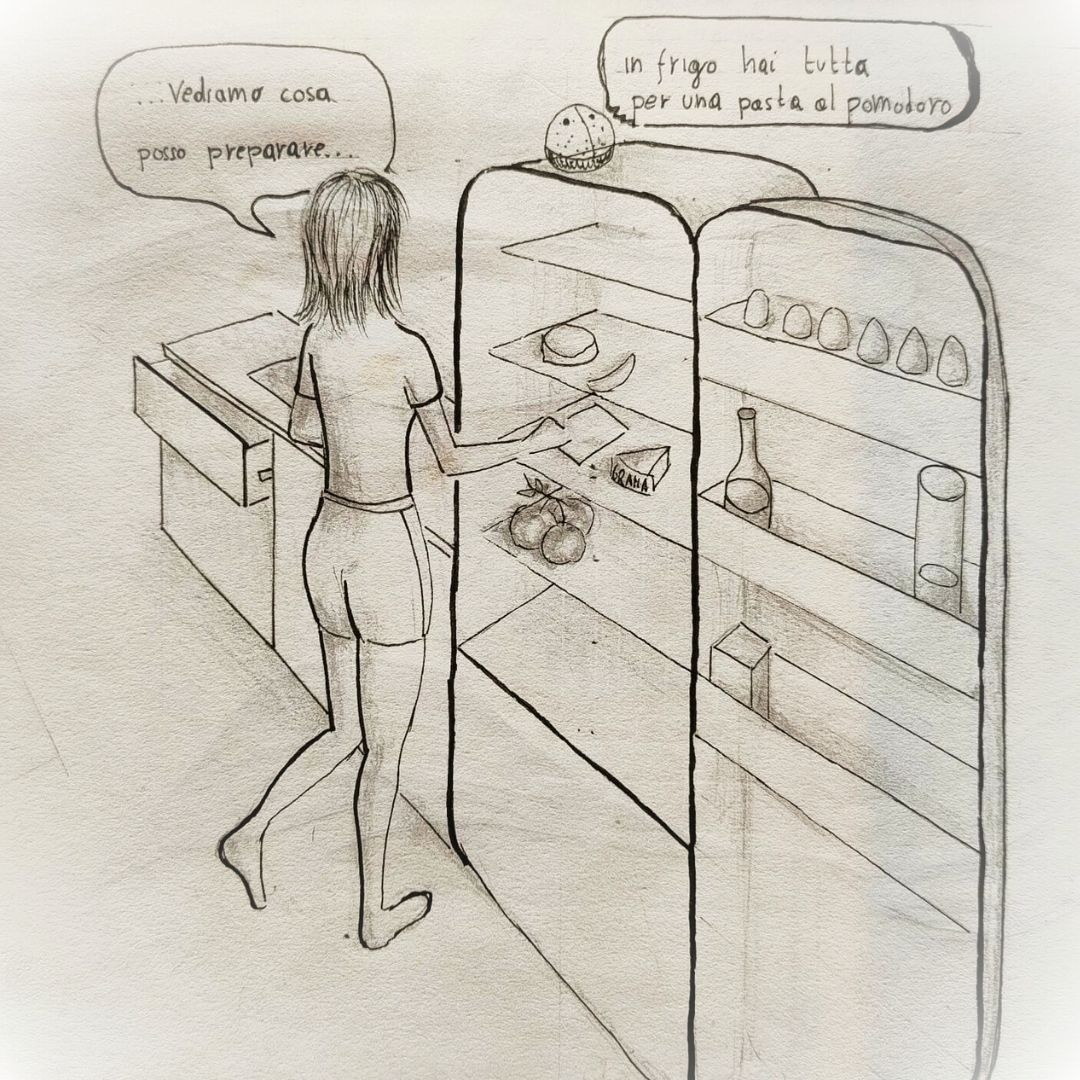
\includegraphics[width=\textwidth]{immagini/cnot_1.jpeg}} % Sostituisci con il nome del file immagine
    
\end{minipage}
\end{center}


Tornai a casa in fretta, consapevole che l'ora di cena si avvicinava rapidamente. \textbf{Rocky} mi accolse scodinzolando energicamente, pieno di vitalità come sempre. Senza neanche cambiarmi i vestiti, presi il guinzaglio per portarlo fuori per una breve passeggiata. Il tempo era limitato: Caterina sarebbe arrivata a breve, ed ero ancora immersa nei pensieri riguardanti il risultato dell'esame.

Avrei potuto ottenere un risultato migliore se avessi approfondito maggiormente lo studio; avevo trascurato diversi dettagli... anzi, non erano semplici dettagli, ma aspetti importanti. Ora, se desideravo mantenere una buona media, avrei dovuto rifare l'esame. Questa consapevolezza mi pesava, un promemoria della necessità di una dedizione ancora più intensa.

Rocky, invece, desiderava giocare, ignaro delle mie preoccupazioni. Cercava di attirare la mia attenzione, ma lo indirizzai gentilmente verso casa. "Dai, Rocky, non oggi..." gli dissi, cercando di non farlo sembrare un rimprovero. Mi guardò con occhi profondi mentre rientravamo. "Domani giocheremo, te lo prometto," aggiunsi, anche se non ero certa che potesse comprendere appieno le mie parole.

\vspace{1em}
\begin{center}Rocky\end{center}
\hrule
\vspace{1em}

Sentivo che qualcosa stava per succedere! Era un formicolio al naso, l'attesa di qualcosa di eccezionale! Per fortuna non avevo perso tempo correndo dietro ad un bastone, ed ora ero pronto per questo evento.\\ 
Erano quasi le... era buio quando arrivò l'amica profumatissima di Laura, ecco cosa era quel pizzicore. C'era un altro odore insieme al suo. Più che di cane avrei detto di fidanzato!
Forse lo aveva portato con sé? Perché non lo faceva entrare? Dove lo teneva nascosto?
L'annusai in ogni angolo ma lui non c'era proprio. Peccato. Avremmo potuto giocare, chissà che tipo è.

Comunque Laura la accolse con un sorriso anche se impegnata negli ultimi preparativi per la cena. La cucina era inondata dal profumo di sugo e spezie che mi facevano salivare in modo incontrollato. "Ciao, Caterina! Vieni, stavo finendo di preparare."

Si tolse la giacca e la sistemò sulla mia poltrona. "Grazie, Laura. Dove sta la tua sorellina?"

Laura girò il mestolo nella pentola. "Valentina? Ah, è con mio zio per un paio di settimane.''

"Poverina, dev'essere dura," rispose Caterina, riflettendo ad alta voce. "da quanto...''

Laura si voltò verso di lei, notando la nota di tristezza nella sua voce.  "Siediti, la cena è quasi pronta." disse evitando di rispondere.

Laura non parlava volentiri dei genitori da quando se ne erano andati.

Caterina  notò un quaderno aperto sul tavolo, pieno di appunti scritti da Laura che  la incuriosirono, così si sedette e provò a leggere qualche riga.
\begin{center}
\begin{minipage}{0.7\textwidth}
    \centering
    \fbox{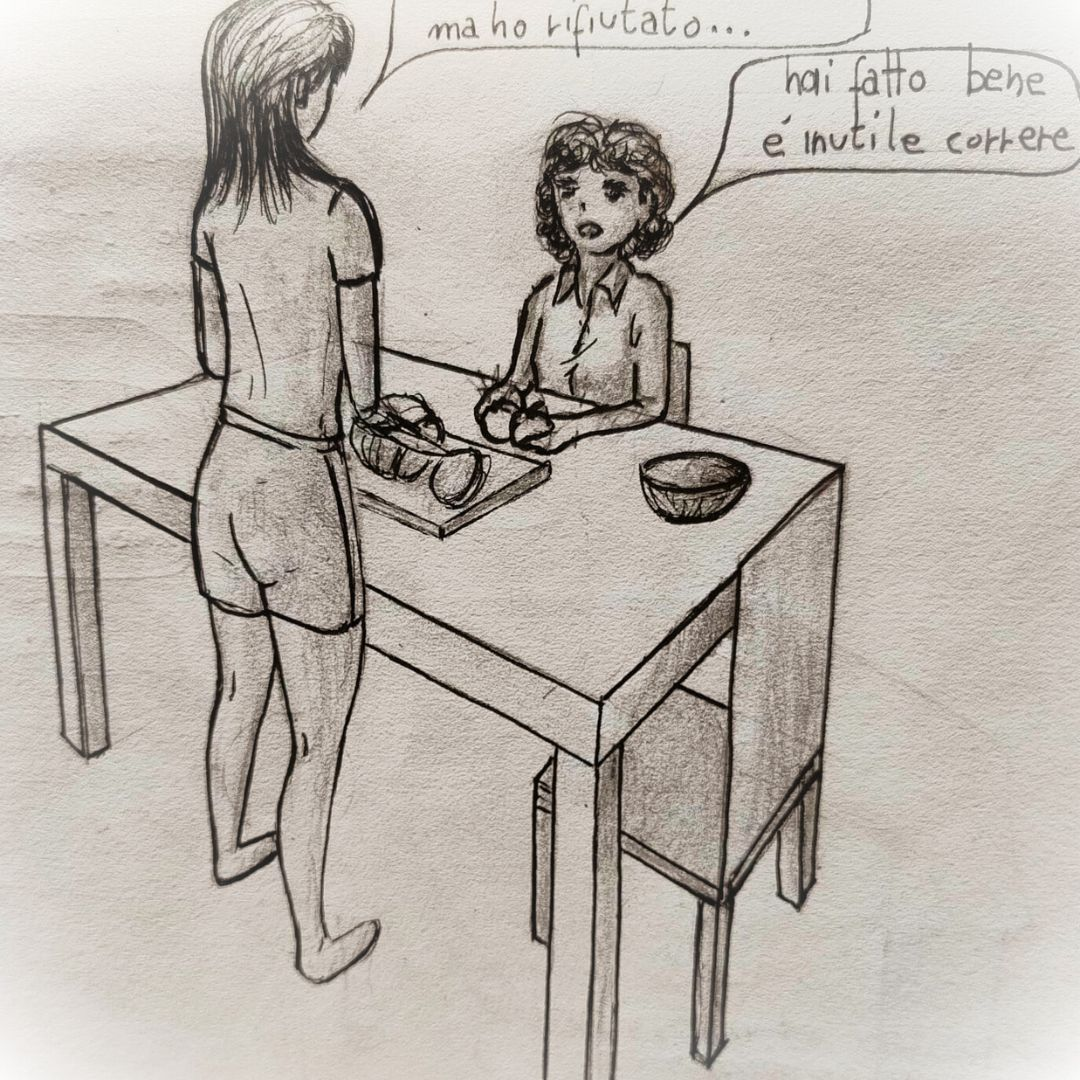
\includegraphics[width=\textwidth]{immagini/cnot_3.jpeg}} % Sostituisci con il nome del file immagine
    
\end{minipage}
\end{center}
\vspace{1em}
\begin{center}Laura\end{center}
\hrule
\vspace{1em}

\begin{dialogue}
\speak{Caterina} \enquote{Wow! Certo che sono proprio complessi questi calcoli.}
\speak{Laura} \enquote{In realtà i calcoli in sé non sono complessi. Si tratta solo di aritmetica, ma è l'idea concettuale che è un po' complicata. Anch'io sto ancora facendo un po' fatica ad appropriarmene veramente.}
\speak{Caterina} \enquote{Ah sì? Eppure mi sembri così brava.}

\speak{Laura} \enquote{Io sono più 'fisica'. La matematica... diciamo che sono più sulla lunghezza d'onda dell'analisi, sai derivate, integrali,  ma l'aritmetica modulare, il calcolo... sono veramente complessi.}
\speak{Caterina} \enquote{Già, ma a volte sono proprio le cose più semplici ad essere più complicate.}
\end{dialogue}

C'era una nota di tristezza nella voce di Caterina. Pensai che forse c'era qualche problema personale di cui non mi voleva parlare.
\begin{dialogue}
  \speak{Caterina} \enquote{Che belle polpette, fanno davvero profumo}.\\
  Le presi la mano e chiusi gli occhi per alcuni secondi. Una eredità della mamma, che prima di mangiare voleva che tutta la famiglia si raccogliesse in preghiera. Quando riaprii gli occhi scoppiai in una risata. Avevo colto Caterina di sorpresa ed era rimasta con la forchetta di fronte alla bocca! Che buffa!
  \speak{Laura} \enquote{Dai, mangiamo} le dissi, e prese forchetta e coltello tagliai un pezzetto di polpetta.
\end{dialogue}


Catarina ogni tanto alzava lo sguardo dal piatto e mi fissava per qualche istante. Sapevo che voleva parlare, ma non trovava il coraggio.

\begin{dialogue}
\speak{Laura} \enquote{Non dirmelo se non vuoi} le dissi strizzandole l'occhio. Cate sorrise e le sfuggì una lacrima
\speak{Caterina} \enquote{Non so, Laura... ho  ricevuto una comunicazione ufficiale dalla \emph{Pet Micro Robot}, ho fallito il colloquio. Sono un po' giù di morale.}

\speak{Laura} Allungai la mano per accarezzarla, \enquote{Non fartene un cruccio, non era sotto il tuo controllo...} 
\speak{Caterina} scosse la testa. \enquote{Credo che la PzIA mi abbia valutata bene, ma Eva, la responsabile delle risorse umane, sembrava intenzionata a farmi crollare. Alla fine anche quel test di programmazione avanzata. Che senso aveva?}

\speak{Laura} appoggiai la forchetta e la guardai perplessa: \enquote{Un test di programmazione per una posizione di marketing... in effetti, è un po' insolito...credo.}

\speak{Caterina} rispose, spingendo il piatto leggermente più avanti. \enquote{Sì, esattamente. Non so perché mi abbia chiesto di fare un test così tecnico. Non mi è sembrato neanche pertinente.}

\speak{Laura} riflettei per un attimo. \enquote{Strano davvero. Forse volevano testare la tua capacità di pensiero logico, ma anche così... è un po' fuori luogo per un ruolo del genere.}

\end{dialogue}
\begin{center}
\begin{minipage}{0.7\textwidth}
    \centering
    \fbox{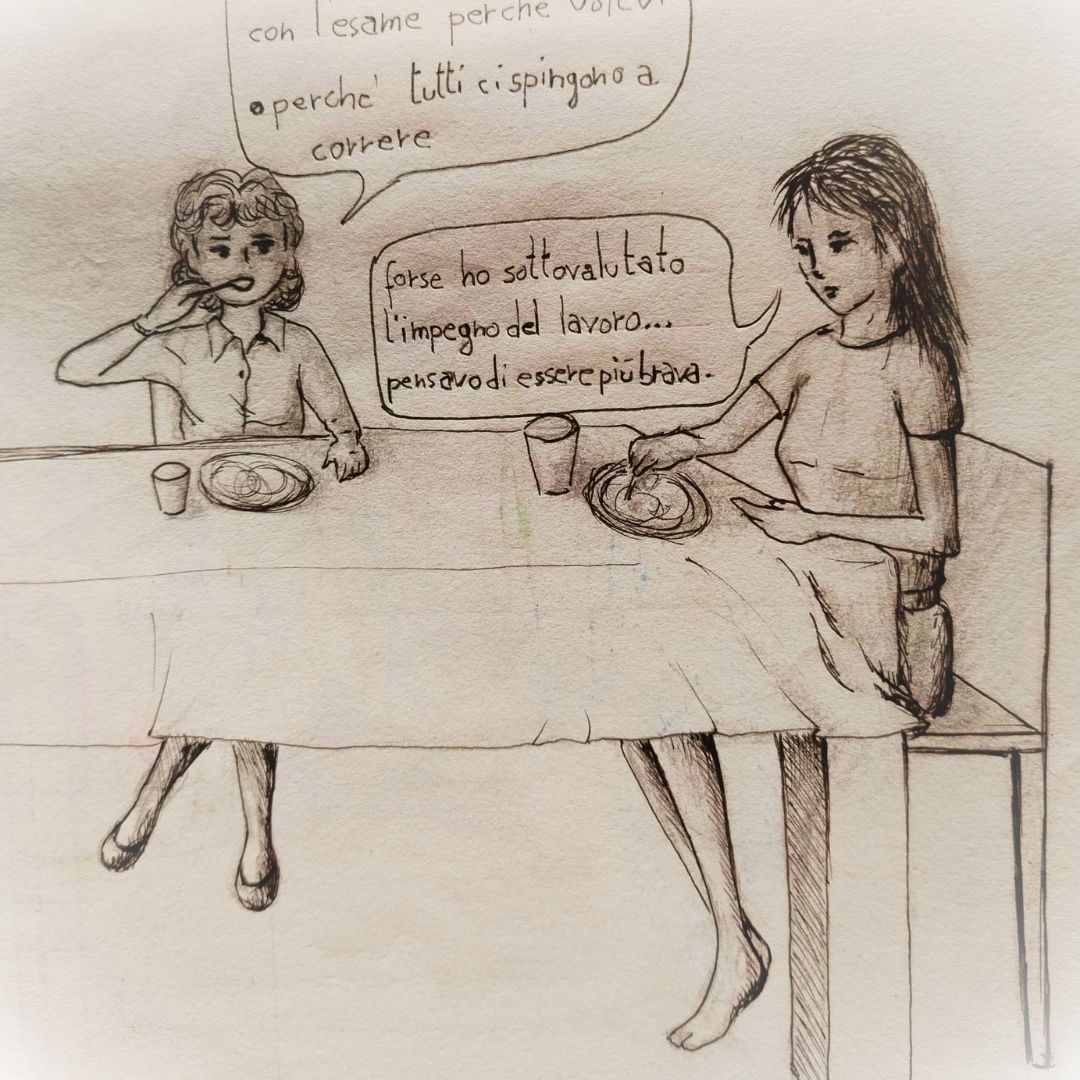
\includegraphics[width=\textwidth]{immagini/cnot_4.jpeg}} % Sostituisci con il nome del file immagine
    
\end{minipage}
\end{center}
\vspace{1em}
\begin{center}Rocky\end{center}
\hrule
\vspace{1em}
Laura e Caterina stavano mangiando. Mangiavano e parlavano. Io volevo uscire, ma loro no, stavano ferme lì. Caterina mi sembrava simpatica e  non l’avevo mai vista giocare. Chissà se sapeva tirare bene la palla. Volevo scoprirlo.  

Le guardavo mangiare insieme senza rubarsi il cibo. Che carine...
Comunque era ora di uscire, in un modo o nell'altro mi sarei fatto capire.

\vspace{1em}
\begin{center}Laura\end{center}
\hrule
\vspace{1em}
Caterina era davvero provata, avrei voluto fare di più ma temevo di risultare inopportuna. Lei è più grande, è già una donna, io sono ancora una ragazza. Cosa  so più di lei per poterla consigliare.
\begin{dialogue}
\speak{Caterina}  \enquote{Mi sembra che questo bel cagnetto si stia agitando. Ha la pipì o sbaglio?}
\speak{Laura} \enquote{Che strano} dissi, \enquote{L'ha fatta solo due ora fa... Comunque possiamo  fare una passeggiata. Cosa dici, abbiamo mangiato abbastanza?}

\end{dialogue}
\enquote{Andiamo} disse Caterina alzandosi da tavola. Mi alzai anche io  diretta verso l'attaccapanni dove tenevo appesi i vari gadget per Rocky.
Alla vista del guinzaglio Rocky si agitò ancora di più, saltellando per la tutta la stanza.

\begin{dialogue}
\speak{Laura} \enquote{Eccoci!} gli disse agganciando il guinzaglio al collare \enquote{Adesso vai un attimo con Caterina mentre chiudo la porta.}
\end{dialogue}

Uscimmo di casa e imboccammo la cappezzagna che dalla via principale porta verso i campi di mais.

\begin{dialogue}
 \speak{Caterina} \enquote{Sai, non imparerò mai a programmare. Tutti questi algoritmi, strutture dati... è tutto così complicato per me.}

\speak{Laura} la guardai e non potei trattenere un sorriso. \enquote{Non dire così. Anche io ho imparato da zero, e non è stato semplice. Ho iniziato da piccola, programmando i vecchi computer di famiglia. Sai, lo \emph{ZX Spectrum} e il \emph{Commodore 64}.}

\speak{Caterina} si fermò un attimo, sorpresa. \enquote{Davvero? Dove li hai trovati?}

\speak{Laura} Mi scappo una risatina. \enquote{Erano cimeli di famiglia, probabilmente di mio zio. Li avevo trovati in soffitta e ho deciso di riportarli in vita. Ho costruito nuovi alimentatori, cavi per i monitor... ed è così che ho iniziato a programmare.}

\speak{Caterina} Mi guardò  stupita. \enquote{Monitor? Pensavo fossero ormai pezzi di antiquariato.}

\speak{Laura} Risi di nuovo: \enquote{sì, lo sono. Ma è stato così che ho imparato. Era una sfida, ma mi ha dato grandi soddisfazioni.}
\end{dialogue}


\begin{dialogue}
\speak{Caterina} \enquote{Certo che le tecnologie sono cambiate veramente tanto da allora. Adesso quasi sembrano cimeli storici.}
\speak{Laura} \enquote{Sì, è vero, la tecnologia sembra diventare obsoleta in fretta, ma in realtà è il marketing della tecnologia che diventa obsoleto.}
\speak{Caterina} \enquote{Cosa intendi?}
\speak{Laura} \enquote{Intendo dire che le persone percepiscono le tecnologie passate come obsolete anche se non ne conoscono i principi di funzionamento. Quindi che senso ha dire che una tecnologia che non conosciamo è obsoleta? Pensa al grammofono. Sapresti spiegarmi come funziona?}
\speak{Caterina} \enquote{Beh, no, direi di no.}
\speak{Laura} \enquote{Non preoccuparti, non volevo metterti in imbarazzo. In realtà quasi nessuno la conosce, anche tra le persone più esperte in tecnologia. È veramente molto interessante. Pensa che il grammofono permette di ascoltare i dischi anche senza alimentazione elettrica.}
\speak{Caterina} \enquote{Wow! Non usa l'elettricità?}
\speak{Laura} \enquote{Non è esatto. Il grammofono produce una piccolissima corrente elettrica dal movimento della testina. Sai cos'è?}
\speak{Caterina} \enquote{Come quella dei giradischi?}
\speak{Laura} \enquote{Esatto, quel segnale elettrico viene trasformato in acustico e amplificato da un corno...}
\speak{Caterina} \enquote{Laura sei così brava! Ma come ha fatto a bocciarti?}
\speak{Laura} \enquote{Beh, forse non sono così brava... comunque io credo che il vero problema sia forse quello di rimanere più legati a tecnologie che possiamo controllare più facilmente, prima di correre troppo avanti.}
\speak{Caterina} \enquote{Cosa intendi? Sicuramente non si può fermare il progresso. Come potresti evitare che qualcuno compri le tecnologie più accattivanti?}
\speak{Laura} \enquote{No, non intendo questo. Però, se si riuscisse a sviluppare più marketing anche attorno a tecnologie più basilari, forse ci sarebbe meno bisogno di battersi per i problemi energetici.}
\speak{Caterina} \enquote{Dici di usare il... come si chiama?}
\speak{Laura} \enquote{Grammofono.}
\speak{Caterina} \enquote{Sì, il grammofono per ascoltare la musica?}
\speak{Laura} \enquote{Sarebbe così brutto?}
\speak{Caterina} \enquote{Non lo so... dovrei provare, ma come credi si potrebbero convincere i consumatori?}
\speak{Laura} Sorrise, \enquote{Non lo so, non sono esperta di queste tecniche.}
\speak{Caterina} \enquote{Però hai ragione,  qui potrebbe entrare in gioco il marketing. Non serve solo a vendere nuove tecnologie, può essere usato anche per far riscoprire il valore di quelle che già esistono. Se raccontassimo meglio i vantaggi del grammofono, come il fatto che non ha bisogno di energia elettrica o che produce un suono unico, potremmo invogliare le persone a usarlo.}
\speak{Laura} \enquote{Quindi,  si tratta solo di cambiare come lo presentiamo?}
\speak{Caterina} \enquote{Esattamente. Alla fine, il marketing crea desiderio. E se potessimo usare quel desiderio per promuovere tecnologie più sostenibili, forse potremmo ridurre l'impatto ambientale senza rinunciare troppo al comfort.}
\speak{Laura} \enquote{Non è una cattiva idea. Forse il grammofono potrebbe davvero tornare di moda!}
\speak{Caterina} \enquote{Ma guarda che è la tua idea! Chissà. Magari un giorno lo vedremo anche nelle pubblicità più cool!}
\end{dialogue}
\begin{center}
\begin{minipage}{0.7\textwidth}
    \centering
    \fbox{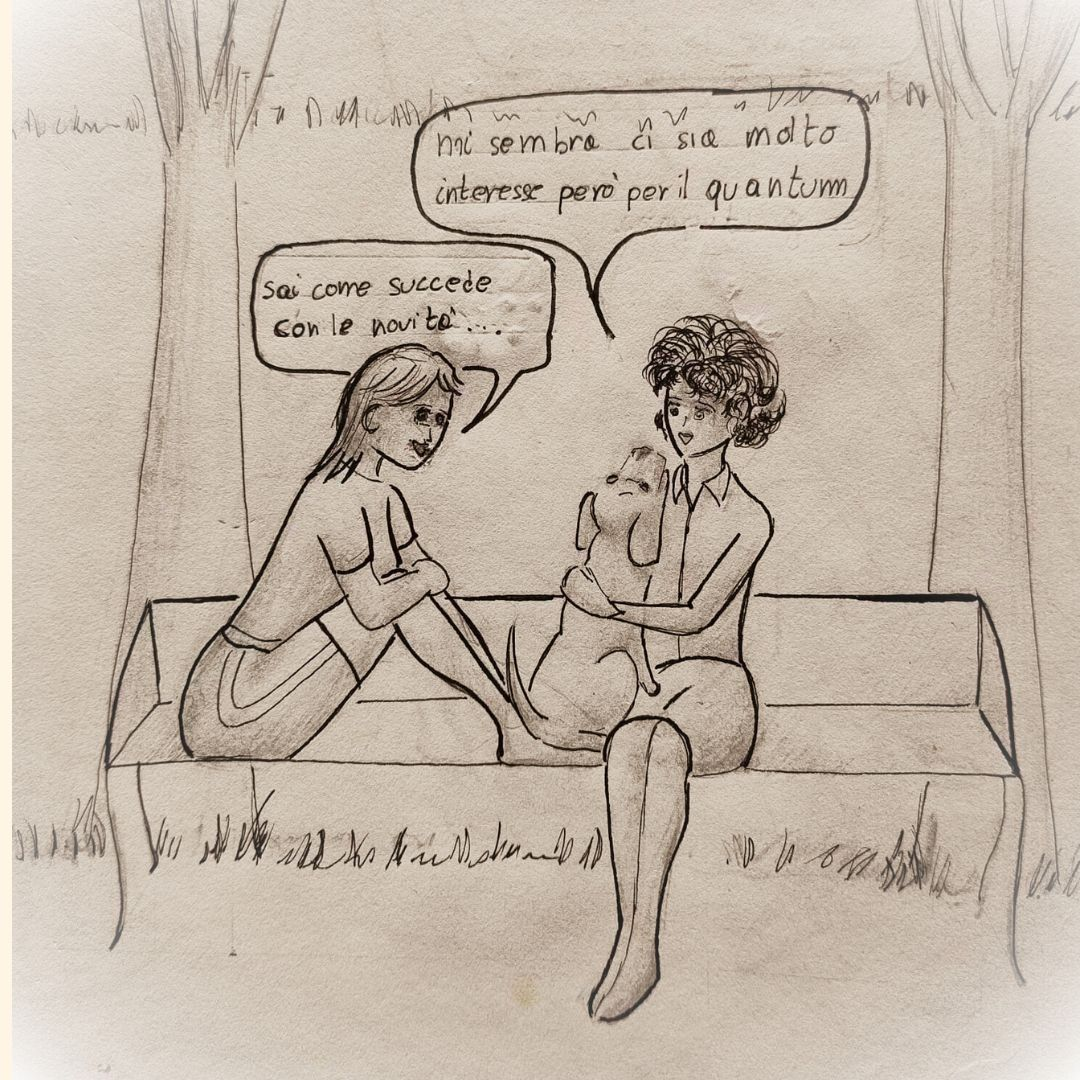
\includegraphics[width=\textwidth]{immagini/cnot_8.jpeg}} % Sostituisci con il nome del file immagine
    
\end{minipage}
\end{center}
La conversazione con Caterina mi aveva rigenerata. In genere quando mi capitava di parlare con qualcuno di temi ``caldi''  come l'energia, l'economia o la tecnologia, era come camminare su un filo sottile sospeso nel vuoto e mi sentivo a disagio.

Non era mai semplice esprimere i miei pensieri. Mi ero abituata alla polarizzazione del pensiero comune, o la pensavi in un modo o nel modo opposto, ma non era quello il mio modo di ragionare. Per questo ogni parola doveva essere ponderata, ogni frase calibrata con precisione, per evitare di finere per essere etichettata. Altrimenti, il risultato era sempre lo stesso: o venivo accusata di essere un'integralista dell'ambiente, come se fossi contraria a ogni forma di progresso tecnologico, oppure mi etichettavano come una negazionista climatica, come se i problemi del pianeta non mi interessassero affatto.


\begin{dialogue}
\speak{Caterina} \enquote{Hai delle idee originali, mi piacciono.}

\speak{Laura} Sorrisi lievemente. \enquote{Probabilmente le mie idee sono troppo slegate dal mondo reale... forse sono un'idealista.}

\speak{Caterina} \enquote{Ma no, non è vero! Forse bisognerebbe provare a far coincidere questi due ragionamenti. Il marketing e i principi possono viaggiare in maniera più unita.}

\speak{Laura} \enquote{In effetti hai ragione. Studiare troppo per compartimenti stagni porta a una visione unilaterale.}

\speak{Caterina} \enquote{Mi piacerebbe parlare ancora con te di questo argomento! Magari potrebbe nascere qualche idea interessante!}
\end{dialogue}

Una sensazione di serenità mi pervase. Il modo in cui Caterina mi aveva ascoltato mi fece sentire compresa. Lei era un'amica con cui potevo dialogare senza timore di essere fraintesa. Mi sentivo a mio agio.

Ci fu un momento di silenzio mentre camminavamo, ma nella mia mente i pensieri continuavano a rincorrersi. Un dettaglio del colloquio di Caterina ed Eva che non mi convinceva del tutto. Un'incoerenza, forse non di natura ``informatica''... piuttosto di natura normativo.

\begin{dialogue}
\speak{Laura} \enquote{Scusami se cambio argomento: sei riuscita a controllare il file di valutazione generato dall'IA?}

\speak{Caterina} Scrollò le spalle. \enquote{Non ho ricevuto nulla}, disse con una nota di rammarico. \enquote{Purtroppo.}

\speak{Laura} \enquote{È strano. Con la nuova legge, tutti dovrebbero ricevere sempre una \emph{chain of thinking} allegata alle decisioni delle IA. Questo mi sembra davvero sospetto}, osservai.

\speak{Caterina} \enquote{Già, non so cosa pensare}, disse, aggiungendo con una punta di frustrazione, \enquote{forse c'è stato un errore...}
\end{dialogue}

Camminammo in silenzio per un po', mentre Rocky scodinzolava felice, ignaro delle preoccupazioni che turbinavano nelle nostre menti. Quella sera era carica di domande senza risposta, ma almeno avevo portato Rocky a spasso.



\begin{tcolorbox}[colback=gray!5,colframe=gray!80,title=\textbf{Scheda Informativa}]
\begin{itemize}
    \item \textbf{Luogo}: Casa di Caterina
    \item \textbf{Ora}: 22:20
\end{itemize}
\end{tcolorbox}

\vspace{1em}
\begin{center}Caterina\end{center}
\hrule
\vspace{1em}

Tornai a casa dopo la passeggiata, ma non riuscivo a rilassarmi. Il pensiero del documento valutativo continuava a tormentarmi incessantemente. Cosa potevo fare? Non mi piaceva l'idea di non avere il controllo su qualcosa di così importante per il mio futuro. Mi sembrava assurdo. Non erano nemmeno in grado di comunicare correttamente un risultato. Che disastro.

Volevo quel posto. Ne avevo bisogno, disperatamente. Non solo perché non sopportavo l'idea di restare a Bamazon per sempre, ma perché era il momento di dimostrare a me stessa di essere all'altezza. Lo dicevano tutti: nel marketing i risultati veri si ottengono nei primi anni, quando si è giovani, quando si ha energia. E se io stavo già fallendo, allora cosa mi restava? Non volevo essere quella che non ce la fa, quella che delude se stessa e gli altri.

Ma c'era anche dell'altro... Non era solo il lavoro a turbarmi. Mi tornavano in mente le parole di Mark. \emph{"Ti confidi più con gli altri che con me."} Forse aveva ragione. Ma cosa significava questo? Perché avevo sempre questa difficoltà a parlare con lui? Era davvero la persona con cui volevo passare il resto della vita? Forse non sono  pronta? Forse non sono abbastanza matura per affrontare tutto questo. Un uomo avrebbe gestito la situazione meglio di me? A volte mi sento troppo fragile, troppo insicura. Troppo \emph{me}.

Entrata in casa, mi tolsi le scarpe e andai in cucina. Avevo bisogno di una tisana, qualcosa che mi calmasse. Scelsi camomilla e melissa, qualcosa di semplice e rassicurante. Preparai l'acqua e riempii la mia tazza preferita. Poi mi sedetti sul divano con la tazza calda tra le mani, cercando di trovare conforto nel calore. I cuscini erano morbidi, accoglienti, ma la mia mente continuava a tormentarmi.

Presi il telefono e iniziai a scorrere le foto di me e Mark. Vacanze, cene, momenti che una volta mi sembravano così felici. Adesso però c'è un distacco che non capisco. Cosa è cambiato? Forse è sempre stato così e io non volevo vederlo. Mi manca quella sensazione di leggerezza, di complicità. Forse è colpa mia. Forse non sono mai stata abbastanza chiara su chi sono e cosa voglio.

Sorseggiai la tisana, cercando di calmarmi. Ma l'immagine di quel documento continuava a balenare nella mia mente. Non potevo sopportare l'idea di non sapere. Non mi piaceva essere lasciata nell'incertezza. Era frustrante.

Mi alzai dal divano e andai al tavolo dove avevo lasciato il laptop. Lo accesi e aspettai con impazienza che si avviasse, tamburellavo nervosamente con le dita sul bordo del tavolo. Quando finalmente lo schermo si illuminò, aprii la casella di posta e iniziai a scrivere un messaggio.

Le mie dita tremavano mentre digitavo. Non volevo sembrare arrabbiata o insicura, ma non potevo neanche essere troppo arrendevole. 

\begin{tcolorbox}[colback=white!95!blue!5, colframe=blue!75!black, title=\textbf{Email di Caterina a Eva}, fonttitle=\bfseries]
\emph{Gentile Eva,\\
Le scrivo riguardo al documento valutativo che sembra essere scomparso dal sistema. Questo documento è molto importante per me, e vorrei capire se è possibile recuperarlo o riceverne una copia. Apprezzo qualsiasi informazione  possa fornirmi al riguardo.\\
Grazie per l'attenzione.\\
Cordiali saluti,\\
Caterina}
\end{tcolorbox}


Rilessi l'email almeno cinque volte. Ogni parola mi sembrava giusta, ma avevo sempre quel dubbio fastidioso: \emph{"È abbastanza professionale? E se il tono fosse troppo duro? O troppo debole?"} Era come camminare su una corda sottile, cercando di non sembrare né arrendevole né aggressiva.

Il mio cuore batteva forte. Sapevo che inviare quell'email significava affrontare le mie preoccupazioni, senza più nascondermi. Ma significava anche espormi. Mi chiedevo se qualcuno al posto mio avrebbe avuto meno esitazioni, meno ansie. Magari Mark avrebbe cliccato su "Invia" senza pensarci due volte. Io invece ero lì, ferma, con il cursore sopra il pulsante, quasi a misurare il tempo.

Presi un respiro profondo, cercando di calmare il nodo che sentivo nello stomaco. \emph{"Devo farlo,"} mi dissi, come se cercassi di convincere me stessa. La mia mano tremava leggermente mentre premevo "Invia".

Osservai il messaggio che spariva nella casella della posta inviata, come se portasse con sé un pezzo della mia ansia. Non era del tutto andata via, ma sentivo un piccolo sollievo. Almeno ora stavo facendo qualcosa. Non restavo ferma a rimuginare.

Chiusi il laptop e mi lasciai cadere sul divano. Non era un gran passo, forse, ma almeno era un passo. \emph{"Ora vediamo cosa succede,"} pensai, prendendo la tazza della tisana. Era tiepida, quasi fredda, ma non m'importava. La bevevo più per abitudine che per gusto, cercando un momento di calma.

La mattina dopo, mentre scorrevo distrattamente il telefono, la notifica di una nuova email mi fece trasalire. Era arrivata la risposta, molto più velocemente di quanto mi aspettassi.

\begin{tcolorbox}[colback=white!95!red!5, colframe=red!75!black, title=\textbf{Risposta di Eva a Caterina}, fonttitle=\bfseries]
\emph{Caterina,\\
purtroppo il documento è stato cancellato per errore, quindi non posso fornirlo. Tuttavia, possiamo fissare un appuntamento domani per discutere di persona.\\
Cordiali saluti,\\
Eva}
\end{tcolorbox}
Sospirai profondamente, fissando le parole di Eva. Non era quello che speravo di leggere. Certo, avrei avuto la possibilità di parlare con lei di persona, ma non potevo fare a meno di chiedermi: \emph{"Sarebbe cambiato qualcosa?"} Mi sembrava tutto così ingiusto, come se stessi sbattendo contro un muro invisibile. Quella risposta non faceva che confermare le mie paure: forse non ero stata abbastanza brava, forse non avevo davvero dimostrato di meritarmi quel posto.

Mi sentivo scivolare in quei soliti pensieri che non portano a nulla. \emph{"Se fossi stata più preparata, più incisiva... forse sarebbe andata diversamente."} Non potevo evitarlo; succedeva ogni volta. Ogni insicurezza riaffiorava, come un'onda che cancellava tutto quello che di buono avevo fatto.

E poi c'era Mark. Pensai a cosa avrebbe detto se gliene avessi parlato: \emph{"Non è colpa tua, sono loro che non capiscono il tuo valore."} Mi avrebbe sorriso, cercando di farmi sentire meglio. Mi voleva bene, ne ero sicura, ma a volte sembrava non vedere quanto fossi complicata dentro. Lui era così diverso da me: diretto, razionale, capace di affrontare le cose senza lasciarsi sopraffare. Io, invece, mi arrovello su ogni dettaglio, ogni sfumatura. A volte mi chiedevo se lui capisse davvero chi sono, ma subito dopo mi sentivo in colpa per averlo pensato.

Sapevo di voler bene a Mark, ma non riuscivo a scrollarmi di dosso quella sensazione di vuoto. \emph{"Lo amo davvero?"} mi chiesi, anche se la domanda mi spaventava. Non volevo perderlo, eppure sentivo che c'era qualcosa che non andava, qualcosa che non riuscivo a definire.

Avevo bisogno di sfogarmi, di parlare con qualcuno che non mi facesse sentire sbagliata. Pensai a Laura. Con lei era diverso. Non c'era bisogno di spiegare tutto, non c'era il rischio di essere fraintesa. Lei ascoltava, e basta. Avevo dato buca a Mark e alle cenetta di consolazione che voleva prepararmi preferendo andare da lei e mi sentii in colpa. Ad ogni modo  avevo  bisogno di respirare, di ritrovarmi anche senza il suo aiuto.

\emph{"Parlerò con Laura,"} pensai, più per convincermi che per altro. Non era un rifiuto verso Mark, né un modo per evitarlo. Volevo solo ritrovare me stessa, e sapevo che Laura avrebbe potuto aiutarmi, anche solo standomi accanto.




\newpage
\begin{tcolorbox}[colback=gray!5,colframe=gray!80,title=\textbf{Scheda Informativa}]

    \begin{itemize}
        \item \textbf{Luogo}: Casa di Laura
        \item \textbf{Giorno}: Mercoledì
        \item \textbf{Ora}: 09:30
        \item \textbf{Situazione}: Caterina passa per un saluto rapido a Laura prima di incontrare Eva alla Pet$\mu$Robots
    \end{itemize}
\end{tcolorbox}

\vspace{1em}
\begin{center}Laura\end{center}
\hrule
\vspace{1em}

\vspace{1em}

Caterina suonò alla porta sul retro che dava direttamente sulla strada. Non mi alzai, ero troppo immersa nel mio progetto, così gridai che la porta era aperta. Cate sembrava un po’ esitante. Forse era colpa mia: il caos del mio angolo di lavoro poteva intimorire. Mi trovò seduta alla scrivania, con uno dei miei vecchi computer acceso, intento a ronzare con i suoi ritmi vintage.

\begin{dialogue}
\speak{Laura} alzai lo sguardo e sorrisi. \enquote{Ciao, Cate, vieni avanti coraggio, anche tu sei mattiniera.}

\speak{Caterina} si sedette sul divano, osservando curiosa la mia attività. \enquote{Ho scritto a Eva. Dice che il documento è stato cancellato, ma mi ha dato appuntamento per oggi. Vedremo cosa mi dirà.}

\speak{Laura} annuii, non ero troppo sorpresa. \enquote{Immaginavo. A volte certi sistemi fanno più danni di quanto dovrebbero.} Poi indicai il vecchio computer sul tavolo. \enquote{Guarda cosa ho rispolverato. Ho deciso di rimettermi su questi vecchi cimeli per prepararmi meglio all'esame di crittografia.}

\speak{Caterina} si sporse in avanti, osservando con interesse. \enquote{Che roba è questa? Non pensavo che si riuscisse ad usarli ancora. Mi sembra di essere tornata negli anni '80.}

\speak{Laura} risi. \enquote{Sì, fa un po' quell'effetto, vero? Sto cercando di collegare uno strumento che stiamo sviluppando nel corso di nanotech, il \emph{noemografo}, a questi vecchi sistemi. Volevo vedere se riesco a farli dialogare.}

\speak{Caterina} aveva solo vagamente sentito parlare del \emph{noemografo}, ma non l'aveva mai visto in azione. \enquote{Il noemografo? Non l'ho mai usato. Come funziona?}

\speak{Laura} mi alzai, andai verso una piccola scrivania laterale e tornai con due strani dispositivi, simili a coroncine. \enquote{È un dispositivo che stiamo sviluppando per leggere i pensieri. Viene usato per applicazioni in nanotech, ma sto provando a integrarlo in questi sistemi per una sfida personale.}

Senza dire altro, porsi uno dei dispositivi a Caterina.
\speak{Caterina}. \enquote{Prova. Io ne indosso uno, tu l'altro. Vediamo se funziona.}

\speak{Caterina} guardò il dispositivo con un misto di curiosità e nervosismo. \enquote{Sei sicura?}

\enquote{Sì, fidati. Non è pericoloso,} dissi, sorridendo. \enquote{In pratica ci colleghiamo per qualche attimo. Puoi sentire i miei pensieri e io i tuoi. Solo per un breve momento, però.}
\end{dialogue}

\begin{center}
\begin{minipage}{0.7\textwidth}
    \centering
    \fbox{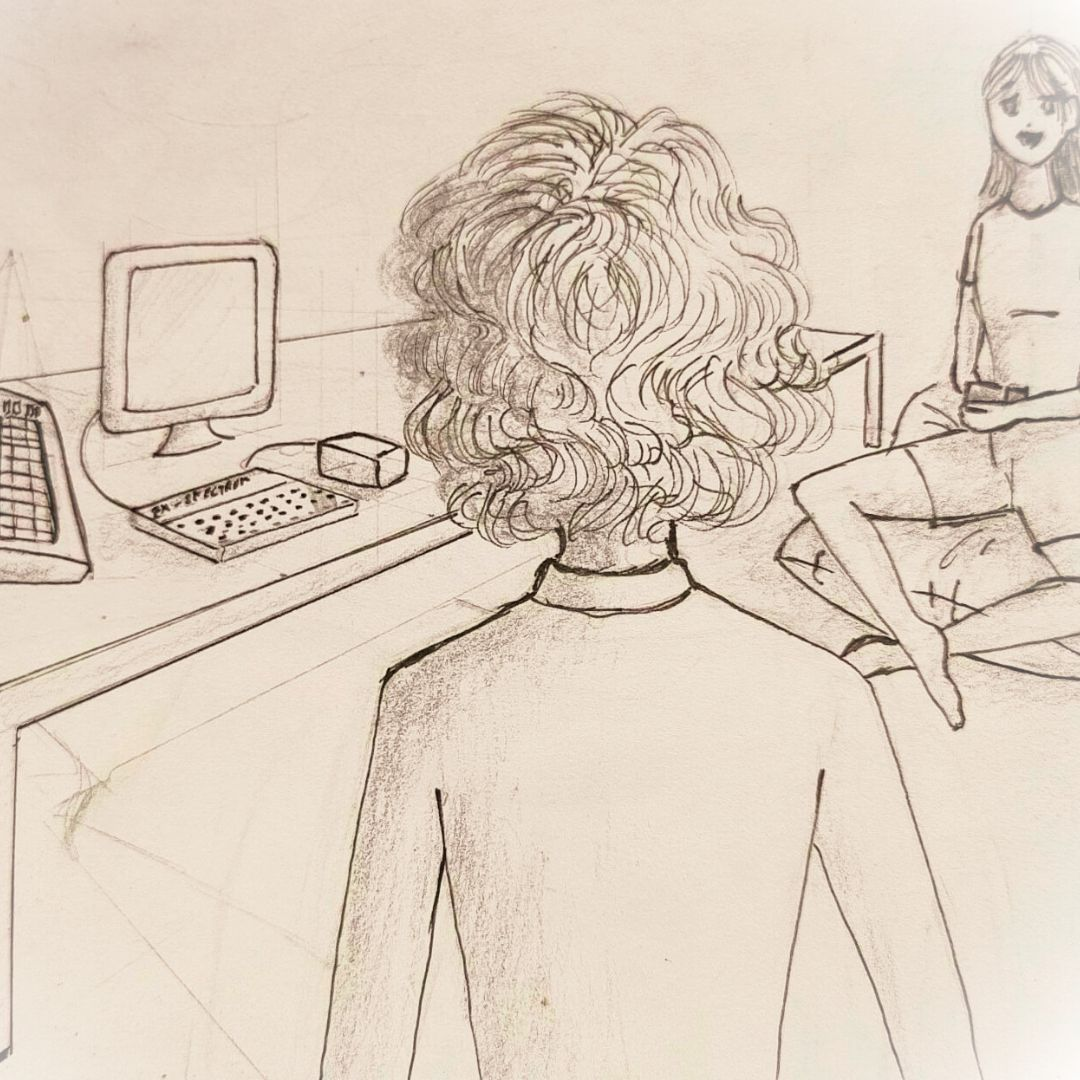
\includegraphics[width=\textwidth]{immagini/cnot_19.jpeg}} % Sostituisci con il nome del file immagine
    
\end{minipage}
\end{center}


Caterina indossò il noemografo, e quasi immediatamente sentii una connessione profonda attraversarmi. Per qualche secondo, le barriere tra noi due si dissolsero. Potevo percepire i suoi pensieri: l'ansia per l'appuntamento con Eva, la frustrazione per il documento cancellato... ma anche qualcosa di più intimo. C'erano frammenti di dubbi e paure legati al suo fidanzato, al matrimonio.

Ero sorpresa, ma decisi di non dire nulla. Quando il collegamento si interruppe, mi limitai a sorridere. \enquote{Funziona, vero?} chiesi con tono casuale, togliendomi il noemografo.

Caterina si tolse il dispositivo e annuì. \enquote{Sì... è stato strano, ma affascinante.}

Feci finta di non aver notato nulla di personale, e forse lei fece altrettanto. \enquote{Beh, è solo un piccolo esperimento. Ma è incredibile quanto la tecnologia possa avvicinarci, non trovi?}

Caterina, ancora un po' scossa dall'esperienza, decise di non parlare dei suoi pensieri. Si limitò a un sorriso vago. \enquote{Sì, lo è. E fra poco... vedremo cosa dirà Eva.}
\begin{center}
\begin{minipage}{0.7\textwidth}
    \centering
    \fbox{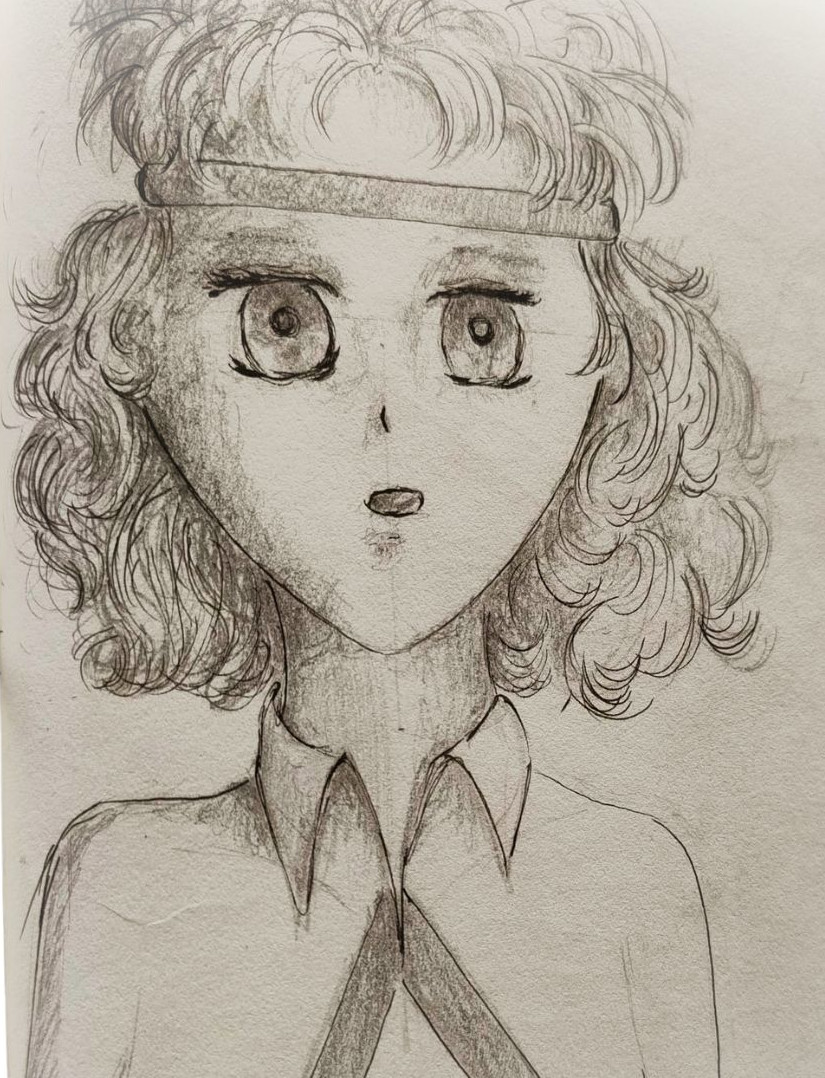
\includegraphics[width=\textwidth]{immagini/cnot_34.jpeg}} % Sostituisci con il nome del file immagine
    
\end{minipage}
\end{center}


\section{La trappola di Eva}

\begin{tcolorbox}[colback=gray!5,colframe=gray!80,title=\textbf{Scheda Informativa}]
\begin{itemize}
    \item \textbf{Luogo}: Reparto Spedizioni, Azienda Bamazon
    \item \textbf{Giorno}: Mercoledì
    \item \textbf{Ora}: 12:30
    \item \textbf{Situazione}: Caterina è al lavoro, preparando gli ultimi pacchi della giornata.
\end{itemize}
\end{tcolorbox}

\vspace{1em}
\begin{center}Caterina\end{center}
\hrule
\vspace{1em}

La mia mente era ancora affollata dai pensieri sul colloquio con Eva e sulla mancanza del file di valutazione. Cercavo di concentrarmi sul lavoro e di mantenere il ritmo, ma sentivo un peso costante che mi opprimeva.

Mentre etichettavo un pacco, ebbi all'improvviso una visione nitida: vidi chiaramente le mani di Laura che digitavano sui tasti di gomma di uno \emph{ZX Spectrum}. Rimasi immobile per un istante, confusa da quella sensazione così precisa e fuori luogo. Non capivo cosa stesse accadendo e scossi la testa per ricacciare quel pensiero. Dovevo tornare al lavoro.

Poco dopo, mi ritrovai a lottare con una spedizione che non riuscivo a completare. Il riferimento del destinatario non funzionava e, nonostante i vari tentativi, non trovavo la soluzione. Alla fine, decisi di chiedere aiuto. Mi avvicinai a Bob e spiegai la situazione.

\begin{quote}
``Non riesco a trovare il corretto riferimento per questa spedizione,'' dissi, mostrandogli il codice sullo schermo. ``Hai modo di darmi una mano?''
\end{quote}

Bob mi ascoltò e si girò verso il suo terminale. ``Sembra un problema complicato,'' disse. ``Meglio chiamare Alice, lei potrebbe avere la soluzione.'' Aprì un canale di comunicazione criptato per evitare rischi legati ai dati sensibili.

Pochi istanti dopo, Alice rispose. ``Ciao, Bob. Che succede?''

\begin{quote}
``Abbiamo un problema con una spedizione,'' spiegò Bob. ``Puoi dare un'occhiata al riferimento? Non riusciamo a collegarlo correttamente.''
\end{quote}

Alice esaminò i dati, ma, dopo diversi tentativi, nemmeno lei trovò una soluzione. ``Mi dispiace, ma potrebbe essere un problema di sistema,'' disse. Sentii crescere la frustrazione.

\begin{quote}
``Grazie lo stesso, Alice,'' risposi con tono calmo. ``Ci proverò più tardi. Devo andare per un appuntamento importante.''
\end{quote}

Bob annuì, e io lasciai il reparto, delusa per non essere riuscita a risolvere il problema.

Il pensiero del file mancante continuava a tormentarmi. Presi un drone taxi e osservai la città scorrere sotto di me. Cercavo di calmarmi, ma un'altra visione apparve nella mia mente: vidi lo schermo dello \emph{ZX Spectrum}, con righe di codice Assembly. Questa volta mi sembrò impossibile ignorarla. Sentivo crescere dentro di me un'inquietudine che non riuscivo a spiegare. Era davvero possibile che io e Laura fossimo ancora connesse attraverso il \emph{Noemografo}? Stavo vedendo quello che stava facendo in quel momento?

Avrei voluto parlarle subito, ma non ne ebbi il tempo. Il drone taxi si fermò, e io scesi. Ero arrivata alla \emph{PET Micro Robot}. Respirai profondamente e mi avviai verso l'ingresso.
\newpage
\begin{tcolorbox}[colback=gray!5,colframe=gray!80,title=\textbf{Scheda Informativa}]

    \begin{itemize}
        \item \textbf{Luogo}: Pet $\mu$ Robot
        \item \textbf{Giorno}: Mercoledì
        \item \textbf{Ora}: 13:15
        \item \textbf{Situazione}: Eva riceve Caterina per chiarire la sua situazione.
    \end{itemize}

\end{tcolorbox}
\vspace{1em}
\begin{center}Eva\end{center}
\hrule
\vspace{1em}
\begin{center}
\begin{minipage}{0.7\textwidth}
    \centering
    \fbox{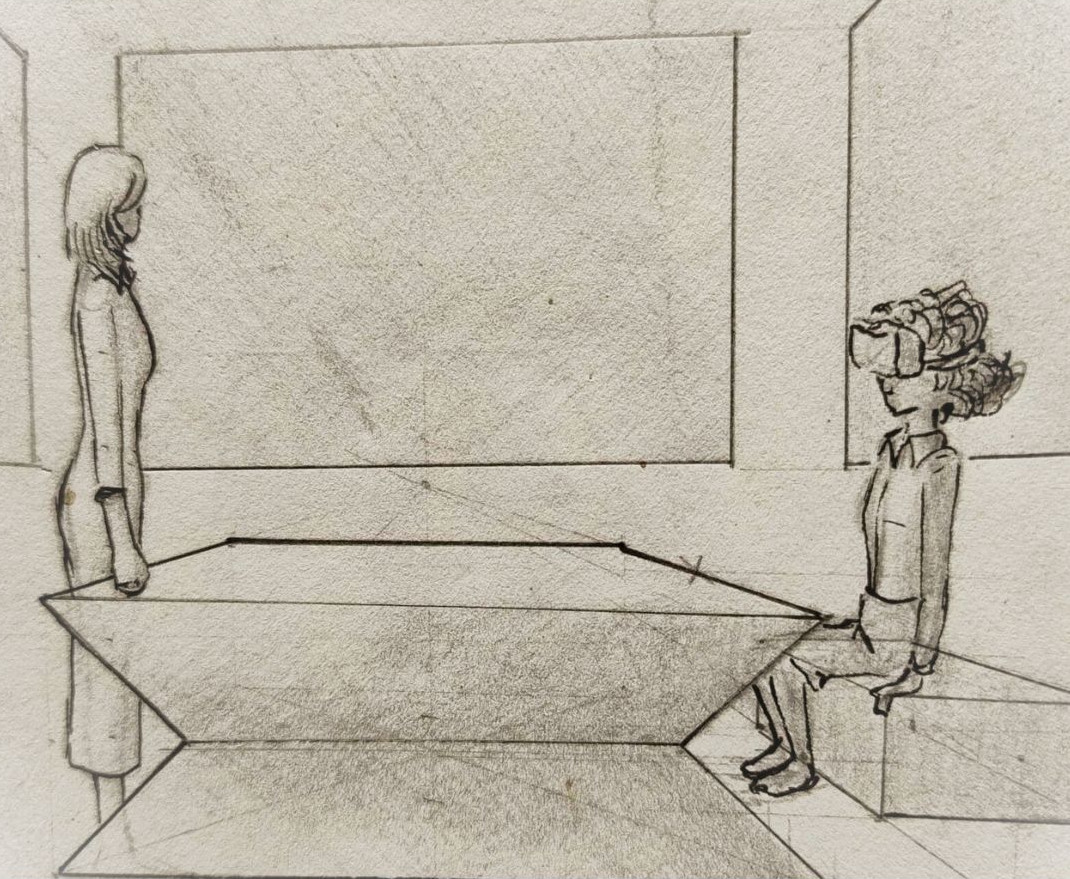
\includegraphics[width=\textwidth]{immagini/cnot_37.jpeg}} % Sostituisci con il nome del file immagine
    
\end{minipage}
\end{center}
Accolsi Caterina con un sorriso calibrato. "Caterina, benvenuta. Mi dispiace per il disguido con il file," dissi con tono professionale. "Comprendo i tuoi dubbi; per questo motivo ho preparato qualcosa che potrebbe rassicurarti."

Mentre annuiva, analizzai le sue reazioni. La tensione nelle spalle e lo sguardo incerto indicavano che non era completamente convinta. Un elemento positivo: il dubbio la rende più ricettiva.

"Ho una registrazione tridimensionale del tuo colloquio, sia con me che con PzIA," continuai, mantenendo un tono neutro. "Per visionarla, dovrai indossare questo visore 3D. È un modello sorpassato, ma ancora utile."

Le consegnai il visore, osservando ogni sua esitazione. Nonostante l'obsolescenza del dispositivo, confidavo che la sua curiosità prevalesse. È incline a cercare risposte, e questo strumento gliele avrebbe apparentemente fornite.

Notai come esaminava il visore, valutando se fidarsi. Rimasi impassibile, attendendo la sua decisione. La pazienza è un'arma efficace: creare le condizioni appropriate spinge gli altri a seguire il percorso stabilito.

Alla fine, Caterina indossò il visore. La vibrazione del dispositivo confermò che tutto procedeva secondo i piani. Lo schermo passò da Augmented Reality a Virtual Reality. Trattenni qualsiasi reazione, ma internamente godevo: ``il mio piano stava funzionando''.


\vspace{1em}
\begin{center}Laura\end{center}
\hrule
\vspace{1em}

Ero seduta alla mia scrivania, avevo scritto un piccolo programma per  lo \emph{ZX}  e lo volevo salvare sul \emph{Micro Drive}.  Mi piaceva la tecnologia della Sinclair, un po' datata ma così originale, lontano dalla complessità che mi circondava ogni giorno.

Stavo per completare l’operazione, ma all’improvviso qualcosa mi colpì. Sentii un vuoto nello stomaco, come se il mio corpo avesse improvvisamente perso peso. Mi girava la testa, e mi sentii instabile sulla sedia. "Che succede?" pensai, ma non c’era una risposta. Mi aggrappai al bordo del tavolo, cercando di stabilizzarmi.

La sensazione era strana, un po' mi preoccupai, ero a casa da sola, chi avrebbe chiamato aiuto se avessi perso i sensi? Non erano solo vertigini: qualcosa mi stava trascinando via, spostandomi da dove ero. Mi sembrava di essere connessa a qualcosa, o a qualcuno. La mia mente andò subito a Caterina: quella mattina non era la prima volta che sentivo una connessione particolare tra di noi.

Mi sforzai di rimanere concentrata, cercando di tornare alla realtà del momento. Ma non potevo ignorarlo: stava succedendo qualcosa, e non era normale. C’era una strana tensione nell’aria, una sensazione che non riuscivo a spiegare. Era come se qualcosa si stesse muovendo tra noi, oltre ciò che potevo comprendere.

Mi lasciai andare contro lo schienale della sedia, respirando profondamente. "Non sono sola in questo," pensai. Sapevo che c’era un legame tra me e Caterina, ma ora sembrava che stesse crescendo, diventando qualcosa di più forte, qualcosa che non potevo ignorare. Tutto divvene nero.



